\chapter[研究二：不干涉匹配时胜率能否计算]{研究二：不干涉匹配时\\胜率能否计算}
\label{ch:winrate}

\begin{answerbox}
\textbf{能算吗？}能算，但算出来的是\emph{期望}胜率，而且它不是实力的单变量函数：胜率由自身实力、实际遇到的对手（和队友）、匹配规则、“胜”的定义和游戏本身的随机性共同决定。随机匹配下有闭式公式（\cref{eq:ch2-random}）：群体实力标准差 200 分时，最强 10\% 的长期胜率约 83\%，最弱 10\% 约 17\%。要从数据上把 52\% 和 50\% 分开，大约需要 4,900 局。

\textbf{和一局的人数有关吗？}有。团队里个人优势被稀释，约按 $1/\sqrt n$（加和模型）到 $1/n$（均值模型）；8 人局的基准率取决于“胜”的定义（第一名 12.5\%，前四 50\%）。

\textbf{和匹配时的段位、分数有关吗？}只通过“配到什么对手”起作用。固定 $K$ 的 Elo 满足精确恒等式“胜率 $=$ 平均预测胜率 $+$ 评分净变化$/(K\times$局数$)$”，按分匹配于是把实力兑换成评分，各实力十分位的胜率被压到 42\%–58\%（匹配窗口约 $\pm100$ 分）或 49\%–51\%（很窄）；评分落后于实力时（新号、回流）胜率才明显偏高。

\textbf{实力是什么？}实力是只在比较中才有意义的潜变量，可操作地定义为“对固定参照池的胜率”。胜率是实力相对实际对手的位置，评分是带噪声、滞后和刻度的估计，两者都只体现一部分实力。

\textbf{实力有波动，还能算吗？}期望胜率仍能算，误差更大：单局独立的波动让胜率曲线变平；自相关的状态起伏让百局胜率的方差变为二项分布的约 1.6 倍（按分匹配，$K=16$）到 3.6 倍（随机匹配），$K=32$ 时约 1.0，实力固定时反而低于二项（约 0.56）；持续进步让胜率比预测高出约“评分上升速度$/K$”。

\textbf{“每局五五开”是什么？}是系统\emph{预测}的胜率为 50\%，即双方\emph{估计}实力相等；真实胜率围绕 50\% 分布，$K=16$ 时 90\% 的“五五开”对局真实胜率落在 38\%–62\% 之间；团队游戏里两队评分和相等，个人对位可以相差很大。
\end{answerbox}

本章所有数值都来自显式模型：玩家实力 $s\sim\Normal(\mu,\tau^2)$（$\mu=1500$，$\tau=200$），1v1 胜率 $p=F(s_i-s_j)$，评分为固定 $K$ 的 Elo，匹配不使用任何隐藏变量。模拟参数在每张图的图注里给出，总表见\cref{app:ch2-params}；代码在 \texttt{code/ch2/}。模型外推到真实游戏时，具体数字会变，但公式给出的依赖关系不变。

% ======================================================================
\section{实力、评分与胜率是三个不同的量}
\label{sec:ch2-defs}

\subsection{实力是只在比较中才有意义的潜变量}

对抗比较模型把每名玩家的实力 $s_i$ 当作看不见的参数：每局里玩家发挥出一个随机的“表现”，表现高者胜，于是 $i$ 胜 $j$ 的概率只取决于实力差，$\Prob(i\text{ 胜 } j)=G(s_i-s_j)$。表现噪声取正态时 $G(x)=\Phi\bigl(x/(\sqrt2\beta)\bigr)$，这是 Thurstone Case~V 模型，也是 TrueSkill 的出发点；取逻辑斯蒂时 $G=F$，即 Bradley–Terry 模型和多数 Elo 变体\cite{herbrich2006trueskill,weng2011bayesian,thurstone1927law,bradley1952rank}\tagLit\needcheck[（Thurstone 1927 与 Bradley–Terry 1952 只核对了书目信息，模型形式依据 TrueSkill 论文和 Weng–Lin 的转述）]。Elo 原书把一名棋手单局表现的标准差定为 200 分，于是两人表现差的标准差为 $200\sqrt2\approx 282.84$\cite{elo1978rating}\tagLit。逻辑斯蒂和正态几乎可以互换：$F(d)\approx\Phi(d/\sigma_d)$，$\sigma_d=1.702/c\approx295.7$，这个系数使两条曲线的最大偏差最小，约 0.95 个百分点\cite{bowling2009logistic}\tagLit；我们在 $|d|\le1500$ 上复核，最大偏差为 0.949 个百分点\tagOwn。本章正文的闭式公式都用这一近似，数值表用精确的逻辑斯蒂积分。

这样定义的实力有三个先天限制：
\begin{enumerate}
\item \textbf{只有差值可识别。}所有人的 $s$ 同加一个常数，任何对局概率都不变。Elo 在原书中写道：“It is only differences on the scale that have real significance in terms of probabilities.”\cite{elo1978rating}\tagLit 所以“实力 1800”只相对某个群体才有意义。暴雪在《守望先锋 2》的匹配说明里也承认，MMR 不是绝对值，个人实力不变时 MMR 也可能因为整体玩家变强或变弱而变化\cite{blizzard2022overwatch}\tagOff。
\item \textbf{刻度由“运气有多大”决定。}Elo 规定 400 分差对应 10:1 的胜负比；TrueSkill~2 的表现噪声 $\beta$ 被明确解释为“反映游戏随机性的参数”\cite{minka2018trueskill}\tagLit。同样的实力差，在随机性大的游戏里换来的胜率更少。
\item \textbf{默认单维、可传递。}存在石头剪刀布式的克制时，单个评分没有预测力；Balduzzi 等人把胜率矩阵分解为可传递部分和循环部分，Elo 只能刻画前者\cite{balduzzi2018reevaluating}\tagLit。卡组、英雄、阵容克制都属于后者。
\end{enumerate}

\subsection{胜率是实力对对手分布的平均}

若玩家实际遇到的对手实力分布为 $\mathcal G$，其长期胜率为
\begin{equation}
  W(s;\mathcal G)=\int F(s-t)\,\dd\mathcal G(t).
  \label{eq:ch2-functional}
\end{equation}
$\mathcal G$ 由群体和匹配规则共同决定。同一个 $s$ 换一个对手池，胜率就变：\cref{fig:ch2-three}(a) 中实力固定为 1756 的玩家，在随机匹配下的胜率随群体离散度从 80.0\%（$\tau=100$）降到 73.2\%（$\tau=300$）；单局随机性变大时降到 73.1\%；换成按分匹配，胜率随匹配窗口收窄从 64.5\% 一路降到 50.9\%\tagOwn。胜率因此不是实力本身，而是“实力相对你实际遇到的对手”。

\begin{figure}[htbp]
  \centering
  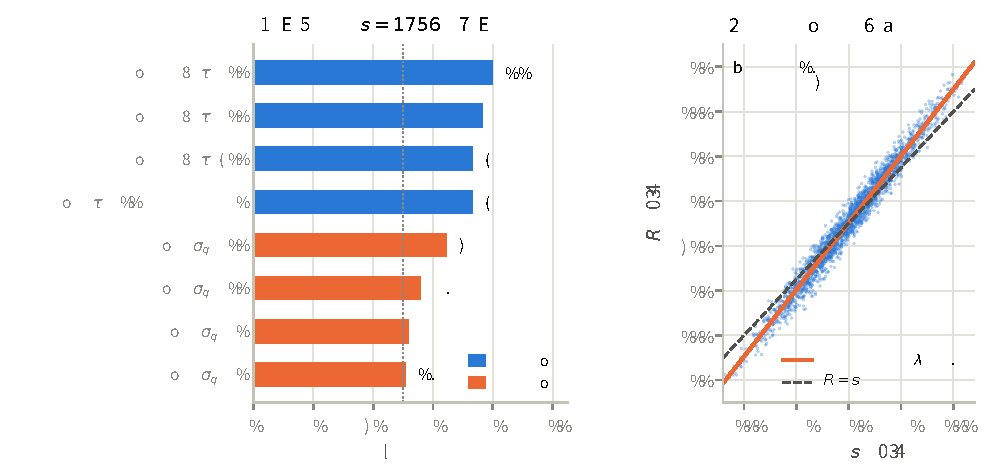
\includegraphics[width=\textwidth]{ch2/three_quantities.pdf}
  \caption{同一实力在不同环境下的长期胜率不同；评分只是实力的带噪声、带刻度的估计。(a) 实力 $s=1756$（$\tau=200$ 群体的第 90 百分位，取实力在 $\pm15$ 分内的玩家平均）在不同对手池和匹配规则下的胜率；(b) 按分匹配（$\sigma_q=100$）第 3000 轮的评分与实力（随机抽 2,500 人作图）。参数：10,000 人，$s\sim\Normal(1500,\tau^2)$，$K=16$，3000 轮，统计第 1001–3000 局。\tagOwn}
  \label{fig:ch2-three}
\end{figure}

\subsection{评分是带噪声、带滞后、带刻度的估计}

TrueSkill~2 的定义很清楚：评分是“根据以往对局结果，对玩家赢下一局能力的估计”，论文还特意区分“玩家的实际实力”和“系统给出的评分”\cite{minka2018trueskill}\tagLit。把评分写成
\begin{equation}
  R_{i,t}=a+\lambda\,s_{i,t}+e_{i,t},
  \label{eq:ch2-rating}
\end{equation}
它与实力之间隔着四样东西：噪声 $e$（标准差 $\sigma_e\approx9.3\sqrt K$，\cref{sec:ch2-sbmm-error}）、滞后（误差衰减需要几十局）、刻度 $\lambda$ 与截距 $a$（零和评分池的整体漂移，以及按分匹配下的刻度伸缩，\cref{sec:ch2-stretch}）。\cref{fig:ch2-three}(b) 是按分匹配稳态下的评分：与实力的相关系数 0.986，排序几乎正确，但斜率 $\lambda=1.19$、残差 41 分\tagOwn。

\begin{keybox}[为什么胜率和分数都只体现一部分实力]
\begin{itemize}
\item \textbf{胜率}衡量的是实力相对“实际对手”的位置。随机匹配下它随实力单调变化，但同时取决于群体离散度和游戏随机性；按分匹配会让对手随你的评分一起移动，胜率便趋于 50\%，几乎不再反映实力（\cref{sec:ch2-sbmm}）。
\item \textbf{评分 / 段位分}衡量的是系统对实力的估计：有 $\pm\sigma_e$ 的噪声、几十局的滞后、随群体漂移的截距，在按分匹配下还可能有被拉伸的刻度；可靠的通常只有排序。可见段位往往还叠加了保底和加分（\cref{sec:ch2-rank}）。
\item \textbf{局内数据}（击杀、伤害、名次分）是另一种局部观测；TrueSkill~2 就把击杀数等作为额外证据\cite{minka2018trueskill}\tagLit，但它们与胜负的关系依赖位置和打法。
\item 可操作的定义：\textbf{实力是能预测“对任意对手胜率”的那个 $s$}。一个可观测的替代量是“对固定参照池的胜率”，在正态群体中它与实力百分位一一对应（\cref{eq:ch2-percentile}）。在按分匹配的数据里，应当从评分和对手评分反推实力，而不是看胜率。
\end{itemize}
\end{keybox}

% ======================================================================
\section{“每局五五开”是预测胜率相等，不是实力相等}
\label{sec:ch2-fair}

\subsection{匹配器拉平的是估计实力，等价于预测胜率 50\%}

匹配器看得到的只有评分。由于 $E=F(R_A-R_B)$ 是评分差的严格单调函数，“双方评分相等”与“系统预测胜率为 50\%”是同一件事；团队游戏里，“两队评分之和（或均值）相等”等价于“团队预测胜率为 50\%”。TrueSkill 用“平局概率”定义匹配质量，并指出“对局质量由结果的不可预测性决定”\cite{herbrich2006trueskill}\tagLit。暴雪说明《守望先锋 2》组局时只看当前 MMR，并称匹配器不会强制任何人 50\% 胜率\cite{blizzard2023overwatch}\tagOff；同一系列的第一篇把“公平对局”直接对应到 50\% 胜率\cite{blizzard2022overwatch}\tagOff。所以“五五开”是关于\emph{系统所掌握的信息}的陈述：在它知道的一切下，分不出谁更强。各厂商原话的逐条对照与“实力五五开、预测胜率五五开、长期胜率五五开”三种读法的辨析见\cref{sec:ch1b-fifty}；本节给出这一读法的数学后果。

\subsection{真实胜率围绕 50\% 分布，宽度由评分误差决定}

\textbf{假设}：评分处于稳态，$R=s+e$，$e\sim\Normal(0,\sigma_e^2)$ 与 $s$ 独立；匹配器把评分恰好相等的两人配成一局。\textbf{推导}：给定 $R$，实力的条件分布是正态，方差 $v=\tau^2\sigma_e^2/(\tau^2+\sigma_e^2)$，两人条件独立，均值相同，于是
\begin{equation}
  \begin{gathered}
  s_A-s_B\mid R_A=R_B\ \sim\ \Normal\!\Bigl(0,\ \frac{2\tau^2\sigma_e^2}{\tau^2+\sigma_e^2}\Bigr),\qquad
  p=F(s_A-s_B),\\
  f_p(x)=\frac{\phi\bigl(F^{-1}(x)/\sigma_\Delta\bigr)}{\sigma_\Delta\,c\,x(1-x)},
  \end{gathered}
  \label{eq:ch2-fair}
\end{equation}
其中 $\sigma_\Delta$ 是实力差的标准差（推导见\cref{app:ch2-fair}）。\textbf{数值}：$K=16$ 时 $\sigma_e=37.7$，$\sigma_\Delta=52.4$，90\% 的“五五开”对局真实胜率在 37.8\%–62.2\% 之间，$|p-\tfrac12|$ 平均 5.9 个百分点；$K=32$ 时 $\sigma_\Delta=73.7$，区间放宽到 33.2\%–66.8\%，平均偏离 8.2 个百分点\tagOwn。从模拟的稳态评分表中把评分相邻的两人配对，得到的区间是 38.3\%–62.1\% 和 33.7\%–66.0\%，平均偏离 5.8 和 8.1 个百分点（\cref{fig:ch2-fair}(a)）\tagOwn。

\begin{figure}[htbp]
  \centering
  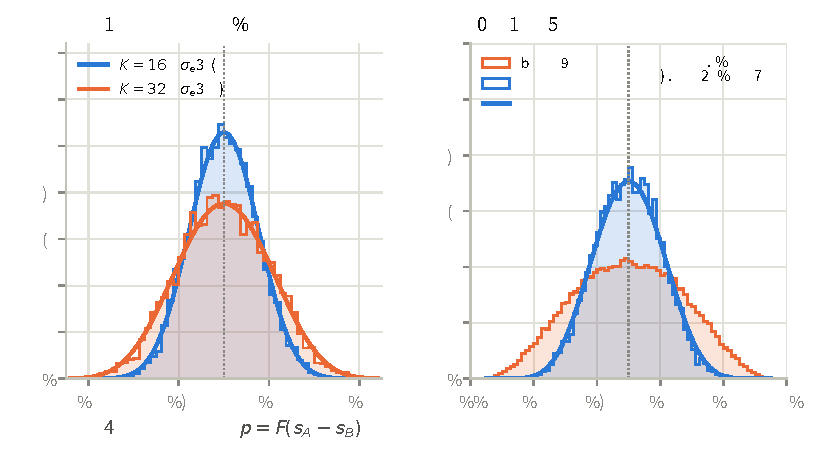
\includegraphics[width=\textwidth]{ch2/fair_game.pdf}
  \caption{“五五开”的一局，真实胜率并不是 50\%。(a) 1v1：把稳态评分表中评分相邻的两人配成一局，直方图为真实胜率 $p=F(s_A-s_B)$，曲线为\cref{eq:ch2-fair}；(b) 5v5（加和模型，$K=16$）：按 $R+\Normal(0,100^2)$ 排序每 10 人一局，在 126 种分队中选评分和最接近的一种，比较团队真实胜率与随机分配位置后的“对位单挑”真实胜率。评分表取自随机匹配模拟第 3000 轮（10,000 人，$\tau=200$）；(b) 重复组局 10 次，共 10,000 局。\tagOwn}
  \label{fig:ch2-fair}
\end{figure}

\subsection{团队游戏：总和相等，个人可以很悬殊}

团队匹配拉平的是两队评分的合计。加和模型下（\cref{sec:ch2-team}）团队实力差为 $(\sum s_A-\sum s_B)/\sqrt n$，给定两队评分和相等时它的方差同样是 $2v$，只是团队游戏中个人评分误差更大（$K=16$、5v5 时约 58 分，\cref{sec:ch2-team}），于是 90\% 的团队对局真实胜率落在 32\%–68\%（模拟 32.8\%–66.9\%）\tagOwn。个人层面更悬殊：以 $\sigma_q=100$ 组局时，一局内 10 人的评分标准差约 84 分，把双方队员随机两两“对位”，90\% 的单挑真实胜率落在 22\%–78\%，约 26\% 的对位偏离 50\% 超过 20 个百分点（\cref{fig:ch2-fair}(b)）\tagOwn。暴雪描述过同一现象：整局是平衡的，但一方高分坦克对上另一方低分坦克，这条对位会“非常一边倒”\cite{blizzard2022overwatch}\tagOff。

\subsection{这不是关于长期胜率的陈述}

“每局预测 50\%”和“长期胜率 50\%”是两件事。随机匹配下每局预测并不是 50\%，长期胜率也不是；按分匹配下两者都接近 50\%，但长期胜率趋于 50\% 的原因是\cref{sec:ch2-identity}的恒等式：实力优势被换成了更高的评分，而不是某种“拉回 50\%”的干预。反过来，真实匹配器也做不到每局恰好 50\%：排队时间要求放宽窗口，天梯两端人少，“没有同水平对手”时预测胜率就会偏离 50\%（\cref{sec:ch2-window}）。

% ======================================================================
\section{1v1 随机匹配：胜率由实力百分位和运气比例决定}
\label{sec:ch2-random}

\textbf{假设}：每局对手从全体中随机抽取，对手实力 $t\sim\Normal(\mu,\tau^2)$，胜率 $F(s-t)$。此时胜负与评分无关，$K$ 只影响评分，不影响胜率。

\begin{derivbox}[随机匹配的闭式胜率]
用 $F(d)\approx\Phi(d/\sigma_d)$，并利用恒等式 $\E\bigl[\Phi(a+bZ)\bigr]=\Phi\bigl(a/\sqrt{1+b^2}\bigr)$（$Z\sim\Normal(0,1)$；证明：$\Phi(a+bZ)=\Prob(Z'\le a+bZ\mid Z)$，而 $Z'-bZ\sim\Normal(0,1+b^2)$）：
\begin{equation}
  W(s)=\E_t\Bigl[\Phi\Bigl(\tfrac{s-t}{\sigma_d}\Bigr)\Bigr]=\Phi\Bigl(\frac{s-\mu}{\sqrt{\sigma_d^2+\tau^2}}\Bigr).
  \label{eq:ch2-random}
\end{equation}
写成实力百分位 $q$（$s=\mu+\tau z_q$）：
\begin{equation}
  W(q)=\Phi(r\,z_q),\qquad r=\frac{\tau}{\sqrt{\tau^2+\sigma_d^2}}.
  \label{eq:ch2-percentile}
\end{equation}
$r^2$ 是固定自身实力、对手随机时，“两人表现差”的方差中由对手实力离散解释的份额（两人都随机抽取时这一份额为 $2\tau^2/(2\tau^2+\sigma_d^2)$，$\tau=200$ 时 0.48）。单局另有独立噪声 $x\sim\Normal(0,\sigma_x^2)$ 时，把 $\sigma_d$ 换成 $\sigma_d'=\sqrt{\sigma_d^2+2\sigma_x^2}$。
\end{derivbox}

\Cref{tab:ch2-tau} 给出不同群体离散度下的数值。注意“前 10\% 平均”要对组内每个人的胜率求平均，不能把组内平均 $z$ 代入公式，后者因为 $\Phi$ 的凹性会偏高（$\tau=200$ 时 83.7\% 对 83.1\%）。

\begin{table}[htbp]
  \centering\small
  \caption{随机匹配 1v1 的长期胜率与群体实力离散度 $\tau$（$\sigma_d=295.7$）。百分位列用\cref{eq:ch2-percentile}；组平均列对组内每人的精确逻辑斯蒂胜率求平均。\tagOwn}
  \label{tab:ch2-tau}
  \begin{tabular}{rrrrrrr}
    \toprule
    $\tau$ & $r$ & $r^2$ & 第 75 百分位 & 第 90 百分位 & 前 10\% 平均 & 前 1\% 平均\\
    \midrule
    100 & 0.320 & 0.10 & 58.6\% & 65.9\% & 71.7\% & 80.7\%\\
    150 & 0.452 & 0.20 & 62.0\% & 71.9\% & 78.5\% & 88.2\%\\
    200 & 0.560 & 0.31 & 64.7\% & 76.4\% & 83.1\% & 92.5\%\\
    300 & 0.712 & 0.51 & 68.5\% & 81.9\% & 88.2\% & 96.4\%\\
    400 & 0.804 & 0.65 & 70.6\% & 84.9\% & 90.8\% & 97.9\%\\
    \bottomrule
  \end{tabular}
\end{table}

\textbf{模拟}：10,000 人、$\tau=200$、$K=16$，每人统计 2,000 局，十分位（按实力把玩家分成十等份）平均胜率依次为 17.0、27.9、35.0、41.2、47.1、52.9、58.8、65.1、72.1、82.9\%，精确积分值为 16.9…83.1\%，差别不超过 0.2 个百分点；前 1\% 为 92.7\%（公式 92.5\%），个人长期胜率的标准差为 19.6 个百分点\tagOwn。$K=32$ 的胜率与 $K=16$ 完全相同，因为同一随机种子下配对和胜负都与评分无关\tagOwn。

\textbf{两个敏感性}（\cref{fig:ch2-random}）：
\begin{itemize}
\item \textbf{群体离散度 $\tau$}：同一百分位，$\tau$ 越大（高手和新手差得越远）胜率越极端。TrueSkill 团队在 Xbox Live 上也观察到，运气型游戏（单局双陆棋、UNO）的实力分布窄，技巧型游戏（拟真赛车）的实力分布宽\cite{herbrich2006trueskill}\tagLit——用本节的话说，就是 $r$ 不同。群体整体变强（$\mu$ 上升）而你不变时，你的百分位下降，胜率也随之下降。
\item \textbf{单局随机性 $\sigma_x$}：$\sigma_x=150$ 时 $\sigma_d'=364$，两两胜率曲线（对实力差）的斜率变为原来的 0.81 倍，随机匹配下 $W(q)$ 曲线的斜率变为 $r'/r=357/415=0.86$ 倍，最强 10\% 从 82.9\% 降到 79.4\%（模拟）\tagOwn。Elo 会把预测胜率校准到观测胜率，所以评分差也按同一比例压缩：模拟中评分对实力的斜率为 0.811（理论 0.813）\tagOwn。评分度量的是“以胜率为单位的实力”。
\end{itemize}

\begin{figure}[htbp]
  \centering
  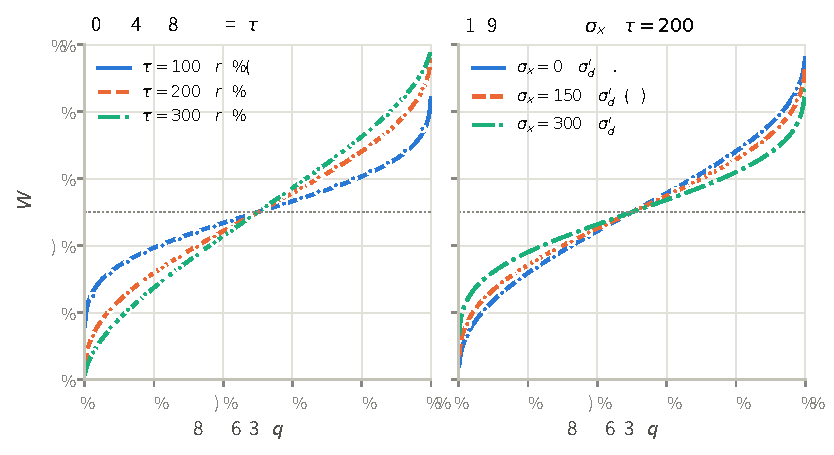
\includegraphics[width=\textwidth]{ch2/random_1v1.pdf}
  \caption{随机匹配 1v1 的长期胜率随实力百分位变化。曲线为\cref{eq:ch2-percentile}，点为模拟（每 5\% 百分位一组的平均胜率）。(a) 群体离散度 $\tau=100/200/300$；(b) 单局独立噪声 $\sigma_x=0/150/300$（$\tau=200$；$\sigma_x=300$ 只画公式）。参数：10,000 人，$K=16$，随机配对，3000 轮，统计第 1001–3000 局。\tagOwn}
  \label{fig:ch2-random}
\end{figure}

随机匹配下评分也能准确恢复实力：Aldous 证明随机配对的 Elo 过程有唯一平稳分布\cite{aldous2017elo}\tagLit，Cortez 与 Tossounian 进一步证明平稳分布以 $\sqrt K$ 的速度集中到真实实力\cite{cortez2024convergence}\tagLit，Olesker-Taylor 与 Zanetti 证明时间平均后的评分以高概率逼近真实参数\cite{oleskertaylor2024analysis}\tagLit。这些定理都假设“谁和谁对局”与当前评分无关；按分匹配不满足这一条件，Jabin 与 Junca 的连续模型显示，只与评分相近者对局时可能出现依赖初值的多个平衡态和很慢的收敛，评分却仍会收敛、看起来一切正常\cite{jabin2015continuous}\tagLit。这正是下一节要处理的情形。

% ======================================================================
\section{1v1 按分匹配：实力被兑换成评分}
\label{sec:ch2-sbmm}

\subsection{一条恒等式说明实力优势去了哪里}
\label{sec:ch2-identity}

固定 $K$ 的 Elo 每局评分变化为 $\Delta R_t=K(y_t-E_t)$。对 $T$ 局求和，$R_T-R_0=K\sum_t(y_t-E_t)$，两边除以 $KT$ 并移项：
\begin{equation}
  W_T\equiv\frac1T\sum_{t=1}^T y_t=\bar E_T+\frac{R_T-R_0}{K\,T}.
  \label{eq:ch2-identity}
\end{equation}
这是代数恒等式，对任何匹配方式都精确成立；在本章所有 1v1 和 5v5 模拟中，左右两边之差不超过 $4\times10^{-15}$\tagOwn。它说明长期胜率偏离 50\% 只有两个来源：一是匹配器系统性地给你更弱或更强的对手（$\bar E\ne\tfrac12$）；二是你的评分还在单向移动（新号、正在进步、刻度在伸缩）。严格按分匹配让 $\bar E\approx\tfrac12$，评分到达稳态后 $R_T-R_0$ 有界，于是 $W_T\to\tfrac12$，偏差按 $1/T$ 衰减：实力强 $\Rightarrow$ 评分高 $\Rightarrow$ 对手强 $\Rightarrow$ 单局胜率回到 50\%。

可变步长时（Glicko 的评分偏差、TrueSkill 的不确定度 $\sigma$\cite{herbrich2006trueskill}、新号阶段放大的 $K$），恒等式变成加权形式 $\sum_tK_t(y_t-E_t)=R_T-R_0$；连胜加分、段位保底等不经过 $K(y-E)$ 的改动会直接打破它。《守望先锋 2》对新号和回流玩家使用的“连胜调节”（胜率高于 50\% 时加快 MMR 上升）就是一种可变步长\cite{blizzard2022overwatch}\tagOff。

\subsection{评分的稳态误差约为 $9.3\sqrt K$，衰减需要 30–65 局}
\label{sec:ch2-sbmm-error}

\textbf{假设}：对手评分与自己相近，各自误差独立同分布。\textbf{推导}：令 $e=R-s$，线性化 $F(s-s')\approx\tfrac12+\tfrac c4(s-s')$，得 AR(1) 型递推
\begin{equation}
  e_{t+1}=\Bigl(1-\frac{Kc}4\Bigr)e_t+\frac{Kc}4e'_t+K\eta_t,\qquad \Var(\eta_t)\approx\tfrac14,
\end{equation}
平稳方差为
\begin{equation}
  \sigma_e^2=\frac{K}{2c\,(1-Kc/4)}\approx\frac{200K}{\ln10},\qquad \sigma_e\approx9.32\sqrt K,
  \label{eq:ch2-sigmae}
\end{equation}
误差的理想时间常数为 $4/(Kc)=1600/(K\ln10)\approx695/K$ 局（推导见\cref{app:ch2-linear}）。\Cref{tab:ch2-sigmae} 给出常用 $K$ 的数值。

\begin{table}[htbp]
  \centering\small
  \caption{Elo 评分误差的线性化数值（$\lambda=1$）。“修正”列含对手误差项；半衰期按离散递推 $-\ln2/\ln(1-Kc/4)$ 计算；“实测”为模拟中误差自相关降到 $1/e$ 的局数。\tagOwn}
  \label{tab:ch2-sigmae}
  \setlength{\tabcolsep}{4.5pt}
  \begin{tabular}{rrrrrc}
    \toprule
    $K$ & $\sqrt{200K/\ln10}$ & $\sigma_e$（修正） & 理想时间常数 $4/(Kc)$ & 半衰期 & 实测衰减时间\\
    &&&&& （按分 $\sigma_q$=100 / 200 / 随机）\\
    \midrule
    10 & 29.5 & 29.7 & 69.5 & 47.8 & —\\
    16 & 37.3 & 37.7 & 43.4 & 29.8 & 55 / 59 / 66\\
    20 & 41.7 & 42.3 & 34.7 & 23.7 & —\\
    32 & 52.7 & 54.0 & 21.7 & 14.7 & 34 / 30 / 34\\
    40 & 58.9 & 60.7 & 17.4 & 11.7 & —\\
    \bottomrule
  \end{tabular}
\end{table}

模拟证实了 $\sqrt K$ 规律：随机匹配下 $K=8,16,24,32,48,64$ 的残差标准差为 26.5、37.8、46.7、54.5、67.9、79.9，公式为 26.5、37.7、46.5、54.0、66.9、78.2（\cref{fig:ch2-error}(a)）\tagOwn。按分匹配下误差略大，因为刻度 $\lambda>1$ 时 $\sigma_e^2$ 按 $\lambda$ 放大（\cref{app:ch2-linear}）。

但 695/K 只是下限。它要求 $\lambda=1$ 且每局 $P(1-P)=\tfrac14$，这两条从不同时成立：随机匹配下对手常常差得远，$P(1-P)<\tfrac14$；按分匹配下配到的对手评分会向均值回归，而且 $\lambda>1$ 会削弱回复力。把这两项写进系数 $\kappa_R=4\E[P(1-P)]\cdot(\lambda\tau^2+\sigma_q^2)/(\sigma_R^2+\sigma_q^2)$（只在本节使用，与第三章的 $\kappa$ 不同），时间常数为 $4/(Kc\kappa_R)$：$K=16$ 时按分匹配为 56–58 局，随机匹配（各人恢复速度不同的混合）为 65 局，实测为 55、59、66 局；$K=32$ 时公式 30–34 局，实测 30–34 局（\cref{fig:ch2-error}(b)）\tagOwn。所以现实的匹配条件下，$K=16$ 的评分误差约 55–65 局才衰减到 $1/e$，$K=32$ 约 30–34 局。这与 Aldous 的看法一致：Elo 在“滞后”和“噪声”之间取舍，$K$ 小则噪声小、滞后大\cite{aldous2017elo}\tagLit。

\begin{figure}[htbp]
  \centering
  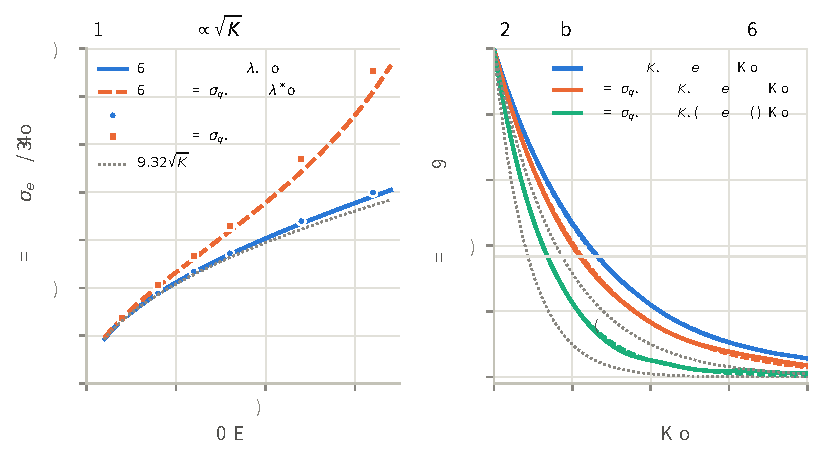
\includegraphics[width=\textwidth]{ch2/rating_error.pdf}
  \caption{评分误差的大小与衰减。(a) 稳态误差（相对评分–实力回归线的残差标准差）随 $K$ 的变化，曲线为\cref{eq:ch2-sigmae}（按分匹配取平稳刻度 $\lambda^*$），点为模拟（4,000 人，2,500 轮，预热 1,000 轮后每 50 轮取一次残差并平均）；(b) 评分误差的自相关：实线为模拟（10,000 人中前 2,000 人第 1001–1400 轮的逐轮评分），虚线为修正后的时间常数，灰色点线为理想值 $695/K$。\tagOwn}
  \label{fig:ch2-error}
\end{figure}

\subsection{匹配窗口决定天梯两端偏离 50\% 多少}
\label{sec:ch2-window}

真实匹配器在一个窗口内找对手。我们用“按 $R+\xi$ 排序后相邻配对，$\xi\sim\Normal(0,\sigma_q^2)$”来模拟，$\sigma_q$ 越大窗口越宽。配到的两人评分差的标准差约为 $\sqrt{2g}\,\sigma_q$（$g$ 见下式）：$\sigma_q=20$ 时约 28 分，系统预测胜率 90\% 落在 43\%–57\%；$\sigma_q=100$ 时约 132 分，预测胜率 90\% 落在 23\%–78\%，已是相当宽松的匹配\tagOwn。

\textbf{推导}（\cref{app:ch2-edge}）：设评分在群体中的标准差为 $\sigma_R$，排序键 $k=R+\xi$，相邻者的键几乎相同。给定自己的评分 $R$，对手评分 $R'$ 服从
\begin{equation}
  \begin{gathered}
  R-R'\sim\Normal\bigl((1-g)(R-\mu),\ g(1+g)\sigma_q^2\bigr),\qquad g=\frac{\sigma_R^2}{\sigma_R^2+\sigma_q^2},\\
  W\approx\bar E\approx\Phi\Biggl(\frac{(1-g)(R-\mu)}{\sqrt{\sigma_d^2+g(1+g)\sigma_q^2}}\Biggr).
  \end{gathered}
  \label{eq:ch2-edge}
\end{equation}
高分玩家平均遇到评分更低的对手，低分玩家相反。这不是操纵，而是“窗口对称、人口密度不对称”的结果，天梯顶端尤其明显；暴雪也提到最高分段“玩家少得多”，组局时更难避免分差\cite{blizzard2022overwatch}\tagOff。

\textbf{数值}（\cref{fig:ch2-sbmm}）：$K=16$ 时最弱到最强十分位的胜率为：随机匹配 17.0\%–82.9\%，$\sigma_q=200$ 时 30.9\%–69.1\%，$\sigma_q=100$ 时 42.1\%–58.0\%，$\sigma_q=50$ 时 47.6\%–52.4\%，$\sigma_q=20$ 时 48.8\%–51.2\%\tagOwn。$K=32$ 的对应值为 31.6\%–68.4\%、43.5\%–56.5\%、48.3\%–51.7\%、48.9\%–51.1\%\tagOwn。\Cref{eq:ch2-edge} 给出的最强十分位胜率为 57.8\%（$K=16$，$\sigma_q=100$，模拟 58.0\%）、69.3\%（$\sigma_q=200$，模拟 69.1\%）、56.7\%（$K=32$，$\sigma_q=100$，模拟 56.5\%）\tagOwn。

用\cref{eq:ch2-identity}分解：$\sigma_q=100$ 时偏离 50\% 的部分几乎全在 $\bar E$ 一项，评分项只有 $\pm0.05$ 个百分点；$\sigma_q=20$ 时 $\bar E$ 只在 49.7\%–50.3\%，剩下的 $\pm0.9$ 个百分点来自评分项，即下文的刻度拉伸，它随时间减小\tagOwn。

\begin{figure}[htbp]
  \centering
  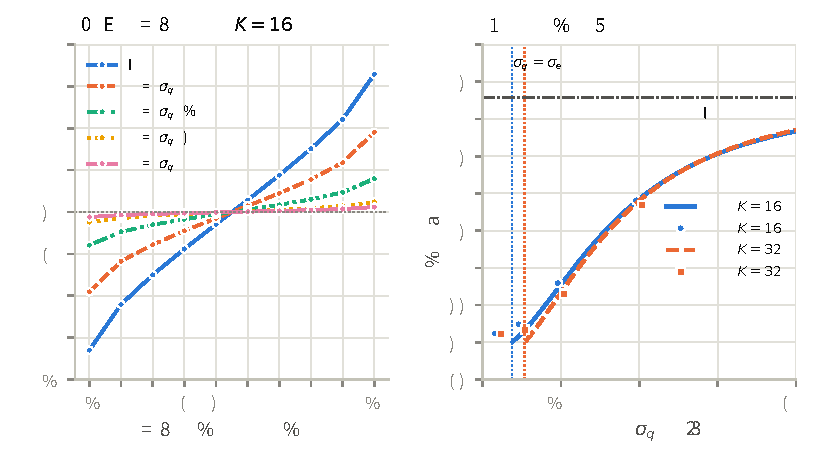
\includegraphics[width=\textwidth]{ch2/sbmm_deciles.pdf}
  \caption{按分匹配把各实力十分位的胜率压向 50\%，压到什么程度由匹配窗口决定。(a) $K=16$ 时各十分位的长期胜率；(b) 最强 10\% 的胜率随匹配噪声 $\sigma_q$ 的变化，曲线为\cref{eq:ch2-edge}（只在 $\sigma_q>\sigma_e$、存在平稳刻度时画出），点为模拟（左右略错开以免重叠），点线标出 $\sigma_q=\sigma_e$。参数：10,000 人，$\tau=200$，按 $R+\Normal(0,\sigma_q^2)$ 排序相邻配对，3000 轮，统计第 1001–3000 局。\tagOwn}
  \label{fig:ch2-sbmm}
\end{figure}

\subsection{新号与回流：强玩家从 1500 起步要几十局才能追回}
\label{sec:ch2-reset}

系统平稳后，从实力前 10\% 中抽 500 人，把评分重置为 1500（相当于高手开新号），跟踪其后 400 局。差距用“实力 $-$ 评分折算的实力”计量，折算用的回归线每轮在未重置玩家上重新拟合。结果（\cref{fig:ch2-reset}）：初始差距约 350 实力分；按分匹配下追回一半需要 47 局（$K=16$）或 30 局（$K=32$），追回 90\% 需要 150 局或 96 局；随机匹配下为 50/191 局和 26/101 局\tagOwn。按分匹配的前 50 局胜率为 77.5\%（$K=16$）和 73.6\%（$K=32$），前 100 局为 72.9\% 和 68.0\%，第 301–400 局回落到 58.9\% 和 57.1\%，即前 10\% 玩家在该窗口下的平稳胜率；随机匹配下胜率与评分无关，始终约 83\%\tagOwn。

两点说明。第一，若把目标线固定在重置前一刻，追回 90\% 看起来要 304 局（$K=16$）和 257 局（$K=32$）：在零和评分池里，把 500 人的评分从约 1920 拉到 1500 会让整个评分池下沉约 20 分，固定目标忽略了这一点\tagOwn。第二，大差距时单局胜率接近饱和，每局最多涨 $K/2$，所以前期比线性理论慢。TrueSkill 在 Xbox Live 上观察到，新玩家若前几局持续输球，整体实力分布会落到先验以下；一次实力重置之后，在更严格的匹配下这一现象消失\cite{herbrich2006trueskill}\tagLit；《守望先锋 2》则通过降低新号初始 MMR 并加快初期调整来处理新玩家胜率偏低的问题\cite{blizzard2022overwatch}\tagOff。

\begin{figure}[htbp]
  \centering
  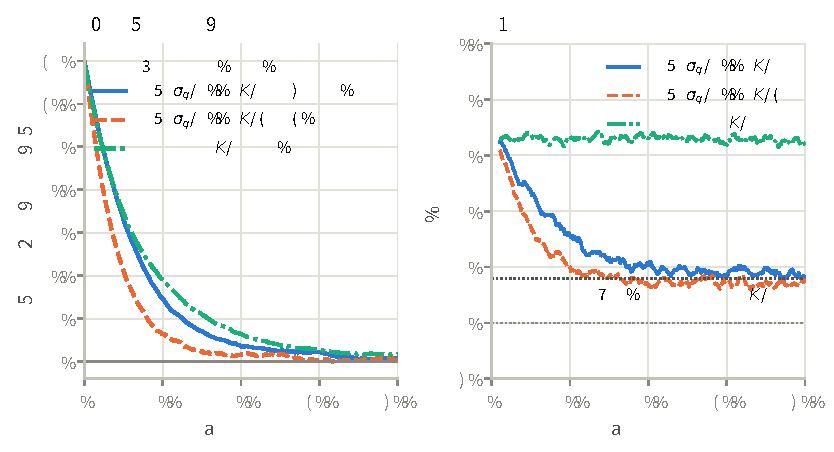
\includegraphics[width=\textwidth]{ch2/reset.pdf}
  \caption{强玩家评分被重置为 1500 后的追分过程。(a) 评分落后于实力的程度（实力分），括号内为追回 50\% / 90\% 差距所需局数；(b) 这批玩家的胜率（10 局滑动平均），点线为按分匹配平稳时前 10\% 玩家的胜率。参数：10,000 人，$\tau=200$，系统运行 1000 轮后从实力前 10\% 中随机重置 500 人，按分匹配 $\sigma_q=100$ 或随机匹配，$K=16/32$。\tagOwn}
  \label{fig:ch2-reset}
\end{figure}

\subsection{严格按分匹配会拉伸评分刻度（理想模型的性质）}
\label{sec:ch2-stretch}

这一节讨论的是本项目在理想模型中推导并模拟出来的性质，\textbf{没有在真实数据中观测到}。

\textbf{精确的出发点}：两名评分完全相等的玩家对局，$E=\tfrac12$，无论谁赢，两人评分都变成 $R\pm K/2$。于是每局使群体评分方差恰好增加 $K^2/4$。只要配对时对手的实力与自己“在给定评分下可交换”，就有 $\Cov(R,\,y-E)=0$，没有任何力量把这部分方差收回。模拟中以 $\sigma_q=0$ 确定性配对 3000 局，评分方差增加 191,792，理论值 $16^2\times3000/4=192{,}000$\tagOwn。方差增加而排序不变，表现为评分对实力的斜率 $\lambda$ 增大，上包络（配对评分完全相等时的理论上限）为 $\lambda(t)^2\approx\lambda_0^2+K^2t/(4\tau^2)$。

\textbf{一般窗口}（\cref{app:ch2-stretch}）：用\cref{eq:ch2-rating}的线性结构做平均场近似（把每名玩家受到的匹配影响换成群体平均），
\begin{equation}
  \frac{\dd\lambda}{\dd t}=\frac{Kc}{4}\cdot\frac{\sigma_e^2+\sigma_q^2(1-\lambda)}{\lambda^2\tau^2+\sigma_e^2+\sigma_q^2},\qquad
  \lambda^*=\frac{1}{1-\sigma_e^2/\sigma_q^2}.
  \label{eq:ch2-stretch}
\end{equation}
分子第一项是“同分对局把评分拉开”，第二项是“窗口内遇到不同评分的对手把刻度拉回”。平稳刻度只在 $\sigma_q>\sigma_e$ 时存在，即配对评分差的标准差要大于约 $\sqrt2\sigma_e$（$K=16$ 时约 53 分，$K=32$ 时约 76 分）。$K=16$ 时 $\lambda^*$ 在 $\sigma_q=50,100,200$ 下为 2.32、1.17、1.04；$K=32$ 时 $\sigma_q=100,200$ 下为 1.41、1.08\tagOwn。模拟（初始评分等于实力，$\lambda_0=1$）第 10,000 局的斜率为：$\sigma_q=20$ 时 3.75（方程 3.77，上包络 4.12），$\sigma_q=50$ 时 2.16 并仍在上升（方程 2.11），$\sigma_q=100$ 时 1.20（1.17），$\sigma_q=200$ 时 1.06（1.04）（\cref{fig:ch2-stretch}）\tagOwn。

\textbf{含义}：刻度被拉伸时排序依然准确（相关系数 0.99），但评分差夸大了实力差，用评分差预测的胜率会过于自信；本章 $\sigma_q=20$ 下各十分位的残余偏离（$\pm0.9$ 个百分点）就是 $\lambda$ 仍在增长带来的评分项。部署中的系统有很多这一模型没有的“锚”：新玩家以默认分进入、赛季软重置、长期不玩后的调整\cite{blizzard2022overwatch}\tagOff、段位保底\cite{blizzard2020developer}\tagOff、排队时间带来的窗口放宽，它们都可能限制拉伸。我们的判断是：无界的 $\sqrt t$ 增长在真实系统中不太可能出现，有界的轻度放大（$\lambda^*$ 在 1.05–1.5 之间）是可能的，但未见实证。

\begin{figure}[htbp]
  \centering
  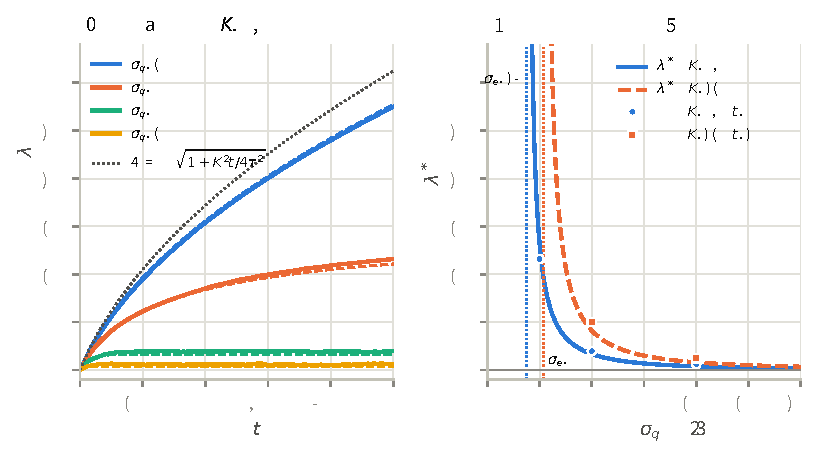
\includegraphics[width=\textwidth]{ch2/stretch.pdf}
  \caption{严格按分匹配下评分刻度的拉伸（理想模型的性质，不是真实数据中的观测）。(a) 评分对实力的回归斜率 $\lambda(t)$：实线为模拟，同色虚线为\cref{eq:ch2-stretch}的平均场方程，灰色点线为配对评分完全相等时的上包络；(b) 平稳斜率 $\lambda^*$ 与匹配噪声 $\sigma_q$，点线为 $\sigma_q=\sigma_e$。参数：(a) 2,000 人，$\tau=200$，$K=16$，初始评分 $=$ 实力，10,000 轮；(b) 圆点取自 (a) 第 10,000 轮，方块取自 10,000 人、初始评分全为 1500、$K=32$ 的模拟第 3,000 轮。\tagOwn}
  \label{fig:ch2-stretch}
\end{figure}

\subsection{可见段位与隐藏分}
\label{sec:ch2-rank}

主流做法是用隐藏分（MMR）匹配，用可见段位提供进度感。暴雪说明《守望先锋 2》组局“从不使用”玩家看到的段位，只看 MMR\cite{blizzard2022overwatch}\tagOff。《炉石传说》酒馆战棋 2020 年起也采用“双评分”：匹配只用内部评分，外显评分叠加保底和进度分\cite{blizzard2020developer}\tagOff（各厂商的做法见\cref{sec:ch1b-blizzard}与\cref{tab:ch1b-disclosure}）。对本章的公式而言，这意味着：
\begin{itemize}
\item 匹配时“段位或分数”影响胜率，只是通过隐藏分决定对手分布 $\mathcal G$；\cref{eq:ch2-identity}适用于隐藏分（若其步长固定）。
\item 可见段位叠加了保底和加分，它的变化不再满足 $K(y-E)$，赛季内会系统性上漂，不宜直接用来估计实力或胜率。
\item 同段位的两个人可能隐藏分相差很大，所以“我和对面段位一样却被碾压”并不与“预测胜率 50\%”矛盾。
\end{itemize}

% ======================================================================
\section{每局人数：团队稀释个人优势，多人局改变基准}
\label{sec:ch2-players}

\subsection{团队游戏：加和模型约按 $1/\sqrt n$ 稀释，均值模型约按 $1/n$}
\label{sec:ch2-team}

\textbf{假设}：焦点玩家比群体平均高 $d$ 分，$n-1$ 名队友和 $n$ 名对手都从 $\Normal(\mu,\tau^2)$ 随机抽取。两种团队模型：
\begin{itemize}
\item \textbf{加和模型}：每名队员有独立表现噪声，团队表现为队员表现之和（TrueSkill 的假设\cite{herbrich2006trueskill}\tagLit），用逻辑斯蒂类比写成 $P=F\bigl((\sum s_A-\sum s_B)/\sqrt n\bigr)$；
\item \textbf{均值模型}：随机性主要在团队层面（地图、阵容、配合），$P=F(\bar s_A-\bar s_B)$。
\end{itemize}
\textbf{推导}：加和模型下自变量 $X=(d+\sum_{n-1}t_i-\sum_n o_j)/\sqrt n\sim\Normal\bigl(d/\sqrt n,\ (2n-1)\tau^2/n\bigr)$，均值模型下 $X\sim\Normal\bigl(d/n,\ (2n-1)\tau^2/n^2\bigr)$，再用\cref{eq:ch2-random}的高斯恒等式：
\begin{equation}
  W_{\text{加和}}\approx\Phi\Biggl(\frac{d/\sqrt n}{\sqrt{\sigma_d^2+(2n-1)\tau^2/n}}\Biggr),\qquad
  W_{\text{均值}}\approx\Phi\Biggl(\frac{d/n}{\sqrt{\sigma_d^2+(2n-1)\tau^2/n^2}}\Biggr).
  \label{eq:ch2-team}
\end{equation}
稀释有两层：个人优势在团队差中只占 $1/\sqrt n$ 或 $1/n$；队友和对手的实力离散 $(2n-1)\tau^2$ 又加了一层噪声。$n$ 较大时，加和模型在 $d=0$ 处的斜率约为 $\phi(0)/\bigl(\sqrt n\sqrt{\sigma_d^2+2\tau^2}\bigr)\propto1/\sqrt n$，均值模型约为 $\phi(0)/(n\sigma_d)\propto1/n$。$n=5$ 时斜率分别是 1v1 的 0.40 和 0.23 倍（$1/\sqrt5=0.45$，$1/5=0.20$）\tagOwn。

\begin{table}[htbp]
  \centering\small
  \caption{随机队友、随机对手时团队人数对个人胜率的稀释（$\tau=200$，精确数值积分）。提升量按 $d=0$ 附近的斜率计算；末列为队友与对手都和群体平均同水平时的加和模型。\tagOwn}
  \label{tab:ch2-team}
  \setlength{\tabcolsep}{5pt}
  \begin{tabular}{rrrrrr}
    \toprule
    & \multicolumn{2}{c}{最强 10\% 的胜率} & \multicolumn{3}{c}{每 100 分优势的胜率提升（百分点）}\\
    \cmidrule(lr){2-3}\cmidrule(lr){4-6}
    $n$ & 加和 & 均值 & 加和 & 均值 & 加和，同水平队友\\
    \midrule
    1 & 83.1\% & 83.1\% & 11.4 & 11.4 & 14.4\\
    2 & 73.9\% & 69.7\% & 7.4 & 6.0 & 10.2\\
    3 & 69.6\% & 64.1\% & 5.9 & 4.1 & 8.3\\
    5 & 65.2\% & 59.0\% & 4.5 & 2.6 & 6.4\\
    6 & 63.9\% & 57.6\% & 4.1 & 2.2 & 5.9\\
    8 & 62.1\% & 55.9\% & 3.5 & 1.7 & 5.1\\
    \bottomrule
  \end{tabular}
\end{table}

\textbf{模拟}（\cref{fig:ch2-team}）：随机分队的 5v5，加和模型十分位胜率为 34.8\%–65.2\%，前 1\% 为 72.8\%，个人长期胜率的标准差 8.8 个百分点（1v1 为 19.6）；均值模型为 41.0\%–59.0\%\tagOwn。哪种模型更接近真实取决于随机性在哪里：TrueSkill 在 Halo 2 的 4v4 夺旗模式中没能胜过 Elo，作者认为可能是因为加和假设不成立\cite{herbrich2006trueskill}\tagLit；TrueSkill~2 发现组队玩家的胜率高于“队员实力之和”所预测的值，于是加入组队偏移\cite{minka2018trueskill}\tagLit。

\begin{figure}[htbp]
  \centering
  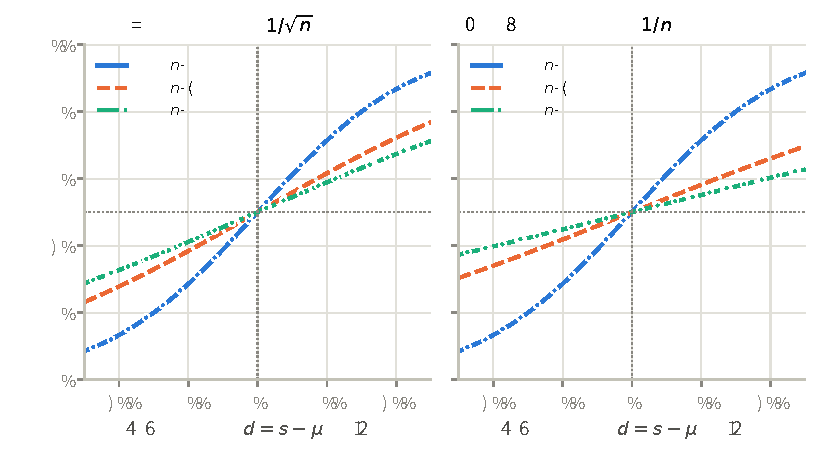
\includegraphics[width=\textwidth]{ch2/team.pdf}
  \caption{团队游戏稀释个人实力优势。焦点玩家比群体平均高 $d$ 分，队友和对手随机。曲线为\cref{eq:ch2-team}对应的精确数值积分；蓝点为 1v1 随机匹配模拟，绿点为 5v5 随机分队模拟（按实力每 50 分一组的平均胜率）。参数：$\tau=200$，10,000 人，$K=16$，3000 轮，统计第 1001–3000 局。\tagOwn}
  \label{fig:ch2-team}
\end{figure}

\textbf{团队的按分匹配}：按 $R+\Normal(0,\sigma_q^2)$ 排序每 10 人一组，组内按评分蛇形分队（从高到低按 ABBAABBAAB 交替选人，使两队评分尽量平衡），$\sigma_q=100$ 时加和模型十分位胜率为 48.7\%–51.3\%，均值模型 48.9\%–51.1\%，$\sigma_q=200$ 时加和模型为 48.1\%–52.0\%；但评分刻度在统计期内一直在拉伸（加和模型 $\sigma_q=100$ 时 $\lambda$ 从第 1000 局的 1.22 升到第 3000 局的 2.04，$\sigma_q=200$ 时从 1.20 升到 1.82），所以这些数字只是某一时刻的快照\tagOwn。分队按评分平衡后，个人实力几乎完全被换成评分；若分队与评分无关（随机分队），十分位胜率要宽得多（\cref{fig:ch2-team}）。团队中个人的评分误差也更大（随机分队）：加和模型的残差为 57.7 分（$K=16$），粗略公式 $\sqrt{K\sqrt n/\bigl(2c(1-\sqrt nKc/4)\bigr)}$ 给出 57.2；均值模型为 84.4 分；1v1 为 37.8 分\tagOwn。

\subsection{多人自由混战：Plackett–Luce 给出名次概率}
\label{sec:ch2-ffa}

\textbf{假设}：$N$ 人一局，表现为实力加 Gumbel 噪声（尺度 $400/\ln10$）。这一设定下，任意两人的相对名次概率恰为 Elo 的 $F$，而完整名次服从 Plackett–Luce 模型：权重（worth）$w_i=10^{s_i/400}$，从剩余玩家中按 $w$ 的比例依次抽出第一名、第二名……\cite{weng2011bayesian}\tagLit（推导见\cref{app:ch2-team}）。\textbf{推导}：焦点玩家对其余 $N-1$ 名同水平对手的优势为 $d$，$w=10^{d/400}$，
\begin{equation}
  \Prob(\text{第 1})=\frac{w}{w+N-1},\qquad
  \Prob(\text{前 }k)=1-\prod_{j=0}^{k-1}\frac{N-1-j}{w+N-1-j}.
  \label{eq:ch2-pl}
\end{equation}
后一式是“前 $k$ 次抽取都没有抽中焦点玩家”的补概率。

\begin{table}[htbp]
  \centering\small
  \caption{8 人自由混战（Plackett–Luce）中，对其余 7 名同水平对手的实力优势 $d$ 与名次指标。\tagOwn}
  \label{tab:ch2-ffa}
  \begin{tabular}{rrrrrr}
    \toprule
    $d$ & $w$ & 1v1 胜率 & 第 1 名 & 前 4 名 & 平均名次\\
    \midrule
    $-200$ & 0.32 & 24.0\% & 4.3\% & 20.8\% & 6.32\\
    0 & 1.00 & 50.0\% & 12.5\% & 50.0\% & 4.50\\
    $+100$ & 1.78 & 64.0\% & 20.3\% & 68.6\% & 3.52\\
    $+200$ & 3.16 & 76.0\% & 31.1\% & 84.6\% & 2.68\\
    $+400$ & 10.0 & 90.9\% & 58.8\% & 98.5\% & 1.64\\
    \bottomrule
  \end{tabular}
\end{table}

\begin{figure}[htbp]
  \centering
  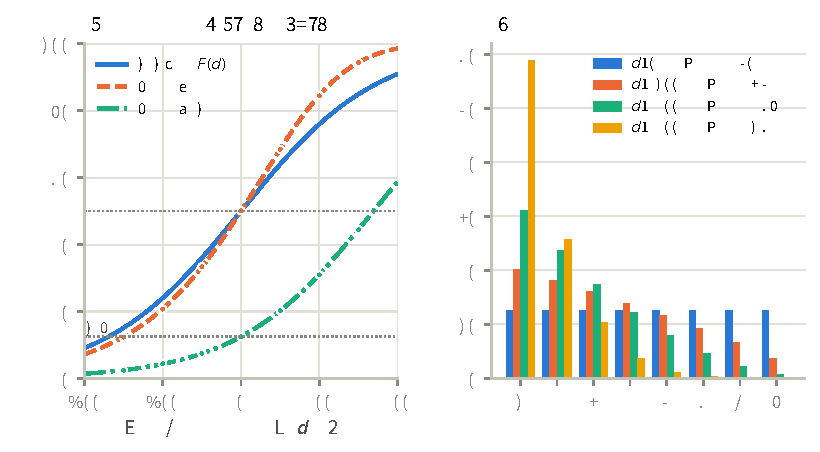
\includegraphics[width=\textwidth]{ch2/ffa.pdf}
  \caption{8 人自由混战中实力优势如何换成名次。(a) 对其余 7 名同水平对手的优势为 $d$ 时进前 4 名和拿第 1 名的概率（曲线为\cref{eq:ch2-pl}，点为 Gumbel 表现的蒙特卡洛，每点 20 万局），蓝线为 1v1 胜率作对照；(b) $d=0/{+}100/{+}200/{+}400$ 时的名次分布。\tagOwn}
  \label{fig:ch2-ffa}
\end{figure}

\textbf{“胜”的定义决定基准率}。按分匹配把同一局 8 人的估计实力拉平，于是均衡时第一名率趋于 $1/N=12.5\%$，前四率趋于 50\%，平均名次趋于 $(N+1)/2=4.5$。模拟（10,000 人，$K=16$，两两 Elo 更新每对步长 $K/7$）：随机组局时最强 10\% 的第一名率 39.8\%、前四率 93.1\%、平均名次 2.20，最弱 10\% 为 1.4\%、10.7\%、6.81；按分匹配（$\sigma_q=100$）时最强 10\% 为 17.0\%、61.3\%、3.90，最弱 10\% 为 8.9\%、39.2\%、5.10\tagOwn。对酒馆战棋这类“前四加分”的游戏，按分匹配下前四率约 50\% 并不说明水平一般；按“第一名”统计，基准是 12.5\%。

\textbf{多人局的评分误差更小}。每局给出 $N-1$ 组两两比较，每组步长 $K/(N-1)$。同水平时名次均匀，单局评分变化的方差为 $K^2(N+1)/\bigl(12(N-1)\bigr)$，而 1v1 为 $K^2/4$；回复力相同，于是 $\sigma_{e,\text{FFA}}=\sigma_e\sqrt{(N+1)/(3(N-1))}$，$N=8$、$K=16$ 时为 24.7 分，模拟为 24.7（按分匹配）和 22.6（随机组局），1v1 为 37.8\tagOwn。酒馆战棋的评分更新同样基于 8 人两两之间的 56 个预测胜率\cite{blizzard2019developer}\tagOff（\cref{sec:ch1b-blizzard}），但具体公式没有公开，本节的两两 Elo 只是常见近似。

% ======================================================================
\section{实力有波动时，期望胜率仍可计算，误差更大}
\label{sec:ch2-fluct}

把当局实力写成 $s_{i,t}=s_i+u_t$。三种波动的后果不同。本节只讨论胜率的水平与方差；“上头”这类由输赢反过来影响状态的反馈，以及它如何制造连败，见\cref{ch:streaks}。

\subsection{独立的单局波动：曲线变平，评分刻度同比例压缩}

$u_t$ 每局独立、标准差 $\sigma_x$ 时，$P=\E\,F(\Delta s+x_i-x_j)\approx\Phi\bigl(\Delta s/\sqrt{\sigma_d^2+2\sigma_x^2}\bigr)$，相当于游戏更随机（\cref{sec:ch2-random}）。Elo 把评分校准到“以胜率为单位的实力”，评分差压缩为实力差的 $\sigma_d/\sigma_d'$ 倍：$\sigma_x=150$ 时理论 0.813，模拟 0.811；随机匹配下十分位胜率 20.6\%–79.4\%，按分匹配（$\sigma_q=100$）下 40.9\%–59.1\%\tagOwn。

\subsection{自相关的状态：评分只吸收一部分，窗口胜率成段波动}
\label{sec:ch2-ar1}

\textbf{假设}：状态服从 AR(1)，$u_{t+1}=\rho u_t+\sqrt{1-\rho^2}\,\sigma_u\varepsilon_t$；取 $\sigma_u=100$，$\rho=0.99$（相关时间约 100 局），作为“状态好坏、疲劳、时段”的示意。

\textbf{评分是指数平滑器}。在实力单位下，Elo 每局把评分朝当局实力移动一个比例 $b=1/\tau_R$（与第三章的 $b$ 同义），即 $\hat s_{t+1}=(1-b)\hat s_t+b(s+u_t)+\text{噪声}$。决定第 $t$ 局胜率的是赛前评分 $\hat s_t$，它对当前状态的回归系数（“被吸收的份额”）为
\begin{equation}
  a=\frac{\Cov(\hat s_t,u_t)}{\sigma_u^2}=\frac{b\rho}{1-(1-b)\rho}.
  \label{eq:ch2-absorb}
\end{equation}
用理想值 $b=Kc/4$ 得 $a=0.70$（$K=16$）和 0.82（$K=32$）；用修正后的时间常数（$\sigma_q=100$ 时 56 局和 34 局）得 0.64 和 0.74，模拟为 0.63 和 0.73\tagOwn。没被吸收的 $(1-a)u_t$ 直接进入单局胜率，所以即使在按分匹配下，“手热”（$u>\sigma_u$）时也多赢：模拟胜率 58.9\%，“手冷”（$u<-\sigma_u$）时 41.1\%；近似公式 $F\bigl((1-a)\E[u\mid u>\sigma_u]\bigr)\approx F(0.36\times152)\approx57.8\%$\tagOwn。

\textbf{逐局几乎看不出，窗口胜率却明显更分散}。按分匹配下逐局结果的自相关只有 0.016（滞后 1 局）、0.014（5 局）、0.008（20 局），很难从单局层面察觉；但 $n$ 局窗口胜率的方差明显偏离二项分布。由\cref{eq:ch2-identity}，窗口胜率的波动来自 $\bar E$ 的局间波动和窗口内评分的净变化，后者的方差由评分对 $s+u$ 的跟踪和评分噪声共同决定，得到（\cref{app:ch2-ar1}）
\begin{equation}
  \begin{gathered}
  \frac{\Var(W_n)}{p(1-p)/n}\approx4\Var(E_t)+\frac{4}{K^2n}\,\Var(R_{t+n}-R_t),\\
  \Var(R_{t+n}-R_t)=2\bigl[\Gamma(0)-\Gamma(n)\bigr],
  \end{gathered}
  \label{eq:ch2-varratio}
\end{equation}
其中 $\Gamma(k)=\lambda^2\gamma_{\hat s}(k)+\sigma_e^2(1-b)^k$，$\gamma_{\hat s}$ 是指数平滑后状态的自协方差。100 局窗口的方差比（模拟/公式）为：随机匹配加状态 3.60/3.80，按分匹配加状态 1.61/1.64（$K=16$）和 1.07/1.01（$K=32$），按分匹配且实力固定 0.56/0.56（\cref{fig:ch2-ar1}）\tagOwn。最后一项小于 1 值得注意：实力固定时按分匹配让胜率比独立抽样\emph{更}稳定，因为评分上涨会立刻带来更强的对手。此时 $\mathrm{sd}(W_n)^2\approx\Var(E_t)/n+2\sigma_e^2(\lambda^*)/(K^2n^2)$：在 $\tau_R\ll n\lesssim500$（$\sigma_q=100$、$K=16$）的范围内第二项占主导，标准差约按 $1/n$ 衰减；局数再多，窗口间“对手运气”的差别 $\Var(E_t)/n$ 不受评分反馈抵消，又回到按 $1/\sqrt n$ 衰减，方差约为二项方差的 0.1 倍（$\sigma_q\to0$ 时这一项消失）。换成“百局胜率不低于 60\% 的窗口占比”，并只看实力接近中位数的玩家（$|s-\text{中位数}|<40$，否则数字主要反映人与人的长期胜率差）：二项分布 2.8\%，按分匹配实力固定 0.7\%，加状态 6.2\%，严格按分匹配（$\sigma_q=20$）0.7\%，随机匹配 4.3\%，随机匹配加状态 17.9\%\tagOwn。Aldous 在三种实力随时间变化的模型中模拟后认为，在他认为合理的参数下，Elo 预测胜率的典型误差不会明显低于 10\%\cite{aldous2017elo}\tagLit；与此一致，状态起伏让“当前胜率”在相当长的窗口里都偏离长期值。

\begin{figure}[htbp]
  \centering
  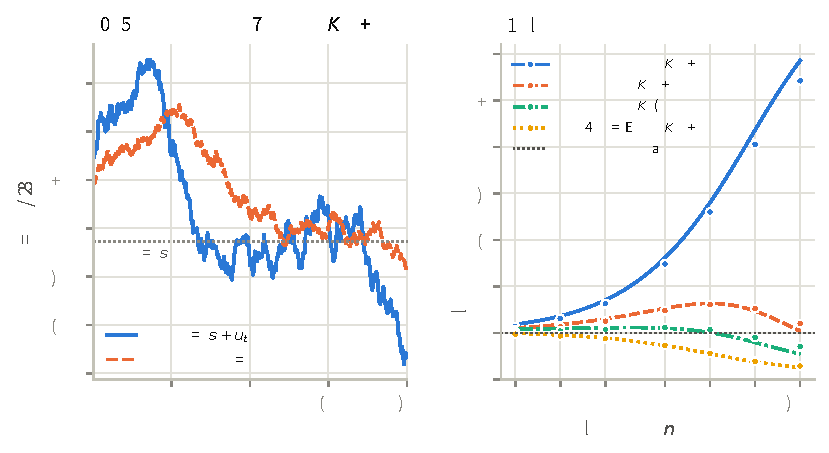
\includegraphics[width=\textwidth]{ch2/ar1.pdf}
  \caption{自相关的状态起伏：评分只能部分追上，窗口胜率比二项分布更分散。(a) 按分匹配（$\sigma_q=100$，$K=16$）中一名实力接近中位数的玩家：当局实力 $s+u_t$ 与评分折算的实力；(b) $n$ 局窗口胜率的人内方差除以二项方差 $\hat p(1-\hat p)/n$，点为模拟（取前 2,000 人的逐局序列，每人 2,000 局切成 $2000/n$ 个窗口），曲线为\cref{eq:ch2-varratio}及随机匹配下的对应公式。参数：10,000 人，$\tau=200$，$\sigma_u=100$，$\rho=0.99$，3000 轮，统计第 1001–3000 局。\tagOwn}
  \label{fig:ch2-ar1}
\end{figure}

\subsection{长期进步：评分滞后，胜率高出期望得分约 $\lambda v/K$}
\label{sec:ch2-improve}

\textbf{假设}：玩家每局实力上升 $v$ 分。\textbf{推导}（\cref{app:ch2-improve}）：由\cref{eq:ch2-identity}，$W-\bar E$ 精确等于评分上升速度除以 $K$。稳态下评分折算的实力与真实实力同速上升，评分以 $\lambda v$ 的速度上升，于是
\begin{equation}
  W-\bar E\approx\frac{\lambda v}{K},\qquad \text{滞后（实力分）}\approx\frac{4\lambda v}{Kc}=\lambda v\cdot\frac{4}{Kc}.
  \label{eq:ch2-improve}
\end{equation}
\textbf{模拟}（\cref{fig:ch2-improve}）：系统平稳后随机抽 2\% 玩家每局进步 $v$，共进步 300 分。按分匹配（$\sigma_q=100$）下，$K=16$ 时 $v=0.25,0.5,1.0$ 的 $W-\bar E$ 为 1.79、3.54、6.67 个百分点，公式（$\lambda^*=1.17$）为 1.82、3.64、7.29；$K=32$ 时为 1.11、2.19、4.40，公式为 1.10、2.20、4.41；$v=0.5$ 的滞后为 28.9 分（$K=16$，公式 25.3）和 15.0 分（$K=32$，公式 15.3）\tagOwn。$v=1$、$K=16$ 时偏低约 9\%，可能的原因是进步者升到高分区后同分对手变少，评分上升受窗口边缘限制。若让 10\% 的玩家同时进步（$v=0.5$），测得的 $W-\bar E$ 会再低 11\%–15\%：进步者之间频繁对局，零和更新不给这一群体带来净分\tagOwn。

真实数据里有对应的痕迹：TrueSkill~2 在 Halo~5 数据中发现，新玩家前 10 局的实际胜率（45\%–47\%）低于经典 TrueSkill 的预测（48\%–49\%），作者把它解释为实力随经验上升、而模型假设实力只做无偏随机游走，并据此加入经验偏移\cite{minka2018trueskill}\tagLit。这正是\cref{eq:ch2-identity}的另一面：胜率与预测胜率的差，衡量的是评分没跟上实力变化的部分。Düring 等人用动理学方程研究了带学习效应的 Elo 模型\cite{during2019boltzmann}\tagLit。

\begin{figure}[htbp]
  \centering
  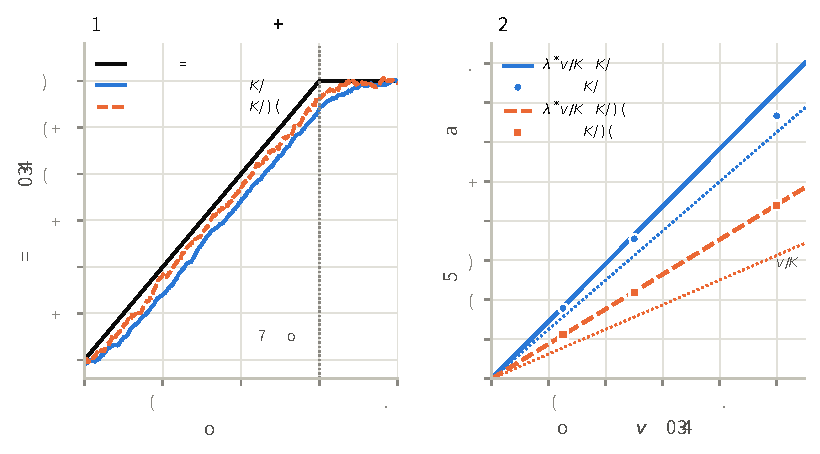
\includegraphics[width=\textwidth]{ch2/improve.pdf}
  \caption{长期进步：评分滞后，胜率高出期望得分。(a) 每局进步 $0.5$ 分的玩家：真实实力增量与评分折算的实力增量；(b) 斜坡第 101 局至结束的 $W-\bar E$，点为模拟，实线为\cref{eq:ch2-improve}（$\lambda^*$ 取 $\sigma_q=100$ 的平稳值），点线为 $v/K$。参数：10,000 人，$\tau=200$，按分匹配 $\sigma_q=100$，系统运行 1000 轮后随机抽 200 人每局进步 $v$、共 $+300$ 分，之后再观察 200 局。\tagOwn}
  \label{fig:ch2-improve}
\end{figure}

\textbf{小结}：实力在变化时，期望胜率仍可写成 $W(t)\approx\bar E(t)+\lambda v(t)/K+\tfrac c4(1-a)u_t$：第一项由匹配决定，第二项来自长期进步，第三项来自没被评分吸收的状态。能算的是期望；不确定性要在二项误差之外乘以\cref{eq:ch2-varratio}的修正因子。

% ======================================================================
\section[统计不确定性：分辨 52\% 与 50\% 约需 4,900 局]{统计不确定性：分辨 52\% 与 50\%\\约需 4,900 局}
\label{sec:ch2-stats}

真实胜率为 $p$ 时，$n$ 局胜率的标准误为 $\sqrt{p(1-p)/n}$：$p=0.5$ 时 20 局 $\pm11.18$、100 局 $\pm5.00$、500 局 $\pm2.24$ 个百分点（一倍标准误）\tagOwn。小样本的区间应使用 Wilson 区间而不是 Wald 区间\cite{wilson1927probable,brown2001interval}\tagLit\needcheck[（Wilson 1927 与 Brown–Cai–DasGupta 2001 只核对了书目信息）]。

\begin{table}[htbp]
  \centering\small
  \caption{观测胜率的不确定性（各局独立）。Wald 半宽按 $p=0.5$ 计算；末列为观测胜率恰为 52\% 时的 Wilson 95\% 区间。\tagOwn}
  \label{tab:ch2-ci}
  \begin{tabular}{rrrr}
    \toprule
    局数 $n$ & 标准误 & 95\% 半宽（Wald） & 观测 52\% 时的 Wilson 区间\\
    \midrule
    20 & 11.18 & $\pm21.9$ & 31.6\%–71.7\%\\
    50 & 7.07 & $\pm13.9$ & 38.5\%–65.2\%\\
    100 & 5.00 & $\pm9.8$ & 42.3\%–61.5\%\\
    200 & 3.54 & $\pm6.9$ & 45.1\%–58.8\%\\
    500 & 2.24 & $\pm4.4$ & 47.6\%–56.3\%\\
    1,000 & 1.58 & $\pm3.1$ & 48.9\%–55.1\%\\
    2,000 & 1.12 & $\pm2.2$ & 49.8\%–54.2\%\\
    5,000 & 0.71 & $\pm1.4$ & 50.6\%–53.4\%\\
    \bottomrule
  \end{tabular}
\end{table}

\textbf{所需局数}。检验 $H_0\colon p=p_0$ 对 $p=p_1$，双侧显著性 $\alpha$、检验力 $1-\beta$ 所需局数为（正态近似，\cref{app:ch2-sample}）
\begin{equation}
  n=\Biggl(\frac{z_{1-\alpha/2}\sqrt{p_0(1-p_0)}+z_{1-\beta}\sqrt{p_1(1-p_1)}}{p_1-p_0}\Biggr)^2.
  \label{eq:ch2-samplesize}
\end{equation}
区分 52\% 与 50\%：$\alpha=0.05$ 双侧、检验力 80\% 需要 4,903 局；单侧 3,862 局；检验力 90\% 需要 6,563 局。若观测胜率恰为 52\%，要让 Wilson 95\% 区间不含 50\%，至少需要 2,401 局\tagOwn。纯运气也会制造“高胜率”：真实 50\% 时，100 局中胜率不低于 60\% 的概率为 2.84\%，20 局中至少 14 胜为 5.77\%、至少 15 胜为 2.07\%，500 局中不低于 55\% 为 1.42\%\tagOwn。玩家基数一大，总有不少人只凭运气就有一段漂亮战绩。

\textbf{相关性会改变误差}（\cref{fig:ch2-ci}(a)）：把\cref{eq:ch2-varratio}的修正因子乘到二项方差上，100 局窗口的 95\% 半宽在按分匹配、实力固定时约为 $\pm7.2$ 个百分点，在随机匹配加状态起伏时约为 $\pm19.7$ 个百分点（相对长期均值），而二项分布为 $\pm9.8$\tagOwn。

\begin{figure}[!tbp]
  \centering
  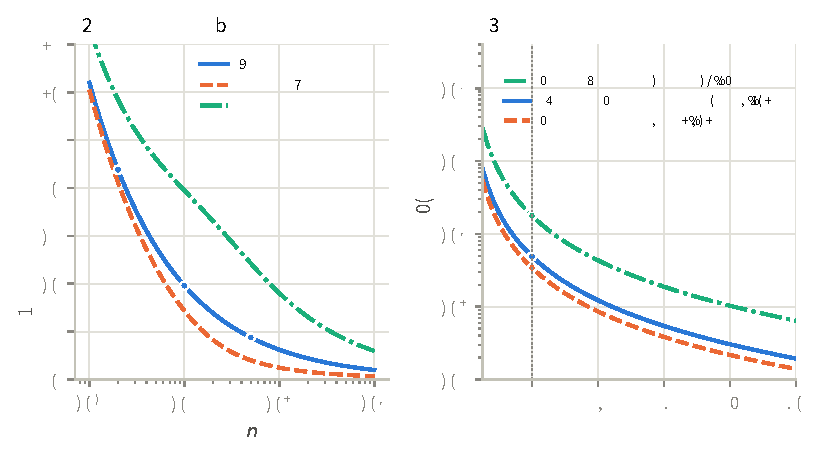
\includegraphics[width=\textwidth]{ch2/ci.pdf}
  \caption{胜率的统计不确定性。(a) 真实胜率 50\% 时 $n$ 局观测胜率的 95\% 区间半宽：二项分布（三个点为 20、100、500 局），以及按\cref{eq:ch2-varratio}修正后的按分匹配（实力固定，$\sigma_q=100$，$K=16$）和随机匹配加 AR(1) 状态（$\sigma_u=100$，$\rho=0.99$）；(b) 双侧 $\alpha=0.05$、检验力 80\% 时区分“五五开”所需局数，8 人局的第一名率与平均名次按 Plackett–Luce 换算到相同的实力优势。\tagOwn}
  \label{fig:ch2-ci}
\end{figure}

\textbf{8 人局}（\cref{fig:ch2-ci}(b)）：前四率是 $p_0=0.5$ 的二项比例，区分 52\% 与 50\% 同样要 4,903 局；第一名率要对 12.5\% 检验，在 Plackett–Luce 下同等实力优势（前四率 52\% 对应 $d\approx11$ 分）的第一名率只有 13.2\%，需要约 17,700 局；平均名次在同水平时的标准差为 $\sqrt{(N^2-1)/12}=2.29$，检测平均名次移动 0.10（4.5→4.4）需要约 4,100 局，而前四率 52\% 的玩家平均名次为 4.39，用平均名次检验只需约 3,400 局\tagOwn。名次本身比“是否进前四”包含更多信息，估计 8 人局实力时应优先用完整名次。


\FloatBarrier
% ======================================================================
\section{小结：胜率能不能算、和什么有关}
\label{sec:ch2-summary}

\Cref{tab:ch2-summary} 汇总本章结论。总的回答是：在“只有输赢、匹配不被操纵”的前提下，胜率可以算，但要先说清三件事——对手从哪里来（随机还是按分）、“胜”指什么（1v1、团队还是名次）、实力是固定还是在变。

\begin{table}[!htbp]
  \centering\footnotesize
  \caption{影响长期胜率的因素：方向与量级（模型参数见各节，$\tau=200$，$K=16$ 除非另注）。\tagOwn}
  \label{tab:ch2-summary}
  \renewcommand{\arraystretch}{1.15}
  \begin{tabularx}{\textwidth}{>{\raggedright\arraybackslash}p{2.6cm}>{\raggedright\arraybackslash}X>{\raggedright\arraybackslash}p{5.2cm}}
    \toprule
    因素 & 方向 & 量级\\
    \midrule
    自身实力（随机匹配） & 实力百分位越高胜率越高，$W=\Phi(r z_q)$ & 最强/最弱 10\%：83\% / 17\%\\
    群体离散度 $\tau$ & 越大胜率越极端 & $\tau$=100→300：前 10\% 由 72\% 到 88\%\\
    游戏随机性 & 越随机越接近 50\%，评分差同比例压缩 & 单局噪声 150：斜率 ×0.81，前 10\% 79\%\\
    匹配规则 & 按分匹配把胜率压向 50\%，窗口越窄越接近 & 十分位范围：随机 17–83\%，$\sigma_q$=100 时 42–58\%，$\sigma_q$=20 时 49–51\%\\
    匹配时的评分/段位 & 只通过对手分布起作用；评分落后于实力时胜率偏高 & 重置的高手前 50 局 77.5\%，约 47 局追回一半\\
    $K$ 因子 & 不改变随机匹配的胜率；决定评分噪声与滞后 & $\sigma_e\approx9.3\sqrt K$；误差衰减 55–65 局（$K$=16）、30–34 局（$K$=32）\\
    每队人数 $n$ & 个人优势被稀释 & $n$=5：斜率为 1v1 的 0.40（加和）或 0.23（均值）\\
    每局人数 $N$ 与“胜”的定义 & 基准率 $1/N$（第一名）或 50\%（前一半） & 8 人局按分匹配：第一名 12.5\%，前四 50\%，平均名次 4.5\\
    独立的单局波动 & 等于游戏更随机 & 见“游戏随机性”\\
    自相关的状态 & 长期胜率几乎不变，窗口胜率更分散 & 百局方差为二项的 1.6 倍（按分）至 3.6 倍（随机）（模拟）\\
    长期进步 & 胜率高于预测胜率 & $W-\bar E\approx\lambda v/K$：$v$=0.5 时约 3.5 个百分点\\
    样本量 & 决定能否分辨 & 52\% 对 50\%：4,903 局（80\% 检验力）\\
    \bottomrule
  \end{tabularx}
\end{table}

\begin{keybox}[本章要点：带到后面两章的三点]
\begin{enumerate}
\item 按分匹配下长期胜率接近 50\% 是\cref{eq:ch2-identity}的直接结果，不需要任何“控胜率”机制来解释；有没有操纵要看匹配输入（\cref{ch:streaks}）。
\item 状态起伏让窗口胜率比二项分布更分散，这是\cref{ch:streaks}讨论连败与“上头”的起点。
\item 从训练的角度看，胜负标签在系统稳定后仍然源源不断，但信息集中在偏离预测的部分（$y-E$），这与\cref{ch:ml}讨论的“目标是胜率还是实力”直接相关。对酒馆战棋这类 8 人名次游戏，评估实力时应使用完整名次而不是前四率，并对固定参照池而不是天梯对手来测量。
\end{enumerate}
\end{keybox}


